
\chapter{Introduction and Literature Review}
\section{Introduction}
Droplet impact is a phenomenon which is prevalent in many industrial processes such ink-jet printing, 
spray cooling of hot surfaces. Microelectronic industries uses precision solder drop dispensing to produce
electric circuits. Aircraft and power distribution lines encounter accumulation of ice involving droplet impact.
Natural phenomena such as rain effects the aeration of lakes, seas and oceans. 
Forensic science necessitates development of non-wettable and fully wettable surfaces. Criminalistics involves
reconstructing crime scenes in which it is need to study the stain patterns of blood drops impacting surfaces.
With a rising world population, there is huge rise in agricultural growth and use of pesticides is necessary. Pesticides spray 
on crops is also an application which exhibits droplet impact on the plants where spreading of droplets is necessary. 
\begin{figure}[tbp]
 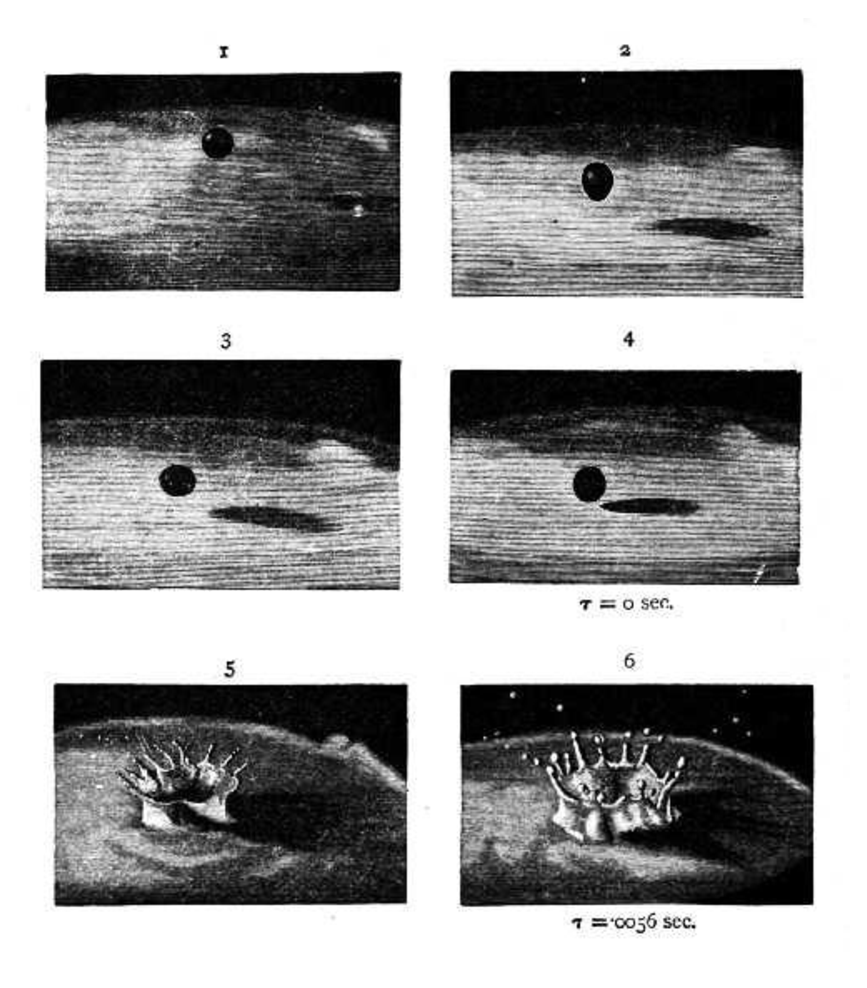
\includegraphics{worthington.eps}
 \caption{Droplet impact graphic by \cite{Worthington1908}}
\label{Fig:Worthington}
\end{figure}


The scientific literature on drops starts with the droplet formation which was studied by many scientists while studying the
free surface flow. The first scientific observation on drops can be found in the book by \cite{Mariotte1700} on motion of  
fluids. They observed that water flowing through the hole of a container bottom breaks into drops. \cite{Taylor1963} solved the  axisymmetric Navier-Stokes  using
singular perturbation method for a drop/bubble in an unbounded fluid. Droplet impact was first investigated experimentally by \cite{Worthington1908} (See Figure \ref{Fig:Worthington}).
The area of droplet formation has also been researched extremely by scientists working in the non-linear dynamics.

The dynamics of the impinging drop is complex and hence many aspects are not understood well. For example, droplets falling
on a surface can undergo many different modes of deformation. It can splash, bounce or simply deposit on a surface. \cite{Rein2002} 
explained through a cartoon, the various possible outcomes of droplet impact. (See Figure \ref{Fig:rein})

\begin{figure}[tbp]
 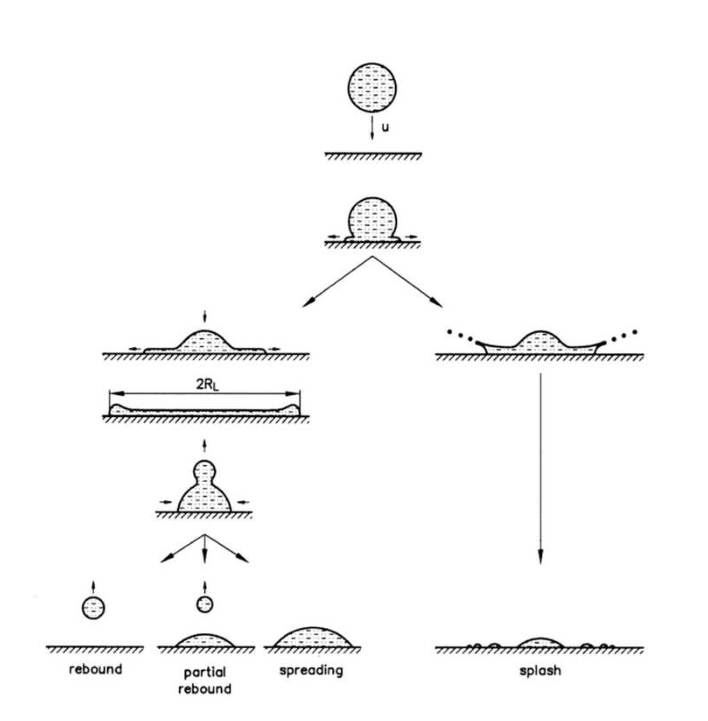
\includegraphics{rein.eps}
 \caption[Different modes of deformation of droplet impact]{Cartoon of different modes of deformation of droplet impact by \cite{Rein2002} }
 \label{Fig:rein}
\end{figure}
